\documentclass{article}

%     \PassOptionsToPackage{numbers, compress}{natbib}
% before loading neurips_2019

% ready for submission
% \usepackage{neurips_2019}

% to compile a preprint version, e.g., for submission to arXiv, add add the
% [preprint] option:
%     \usepackage[preprint]{neurips_2019}

% to compile a camera-ready version, add the [final] option, e.g.:
     \usepackage[final]{neurips_2019}

% \usepackage{neurips_2019}

% to avoid loading the natbib package, add option nonatbib:
%     \usepackage[nonatbib]{neurips_2019}

\usepackage[utf8]{inputenc} % allow utf-8 input
\usepackage[T1]{fontenc}    % use 8-bit T1 fonts
\usepackage{hyperref}       % hyperlinks
\usepackage{url}            % simple URL typesetting
\usepackage{booktabs}       % professional-quality tables
\usepackage{amsfonts}       % blackboard math symbols
\usepackage{nicefrac}       % compact symbols for 1/2, etc.
\usepackage{microtype}      % microtypography
\usepackage{graphicx}       % figures

\title{Beyond Confidence: Learning to Abstain in Wildlife Classification Under Distribution Shift}

\author{%
  John ~Uzodinma
   \And
   Ramsey Njema \\
   \AND
   Emmilly Namuganga \\
   \And
   Stephen N'nouka \\
}

\begin{document}

\maketitle

\begin{abstract}
Automated wildlife monitoring relies on image classifiers to identify animals in
camera-trap photographs, but changes in backgrounds, lighting, and camera placement make
predictions unreliable at unseen locations. Before studying selective
classification---allowing a model to abstain---on iWildCam-WILDS, we establish the fixed
classifier that the abstention mechanism will build on. Following the WILDS iWildCam
leaderboard, we implement and evaluate four baseline families on the official protocol:
CLIP ViT-B/16 fine-tuned with FLYP and with AutoFT (the current \#1 leaderboard method,
which we reproduce faithfully, including its WiSE-FT ensembling step), a ResNet-50 trained
with a robust optimizer (AbsGD, three seeds, two normalization variants), and a CLIP
ViT-H/14 from the Data Filtering Network family. All runs are tracked in Weights \&
Biases under leaderboard-entry naming. AutoFT improves OOD-test macro F1 by +4.0 over
FLYP on the same backbone, and by +6.3 when ensembled with the zero-shot model---matching
the published pattern (+2.7/+6.0) on a smaller backbone. A distributionally robust
ResNet-50 trails the CLIP fine-tunes by 2--10 macro-F1 points, while the DFN ViT-H/14 is
the strongest single model (OOD-test macro F1 46.1). The frozen AutoFT classifier, the
leakage-free location partition, and the full evaluation harness are now in place for the
selective-classification phase, which reproduces and extends Heng \& Soh's
likelihood-ratio abstention baseline.
\end{abstract}

\section{Introduction}
Camera traps help ecologists monitor wildlife by collecting large numbers of animal
photographs. Automated classification can reduce the effort required to label these images,
but models deployed at new camera locations encounter changes in lighting, vegetation,
backgrounds, and viewing angles. These changes can produce incorrect predictions that
nevertheless receive high confidence. Identifying such predictions and flagging them for
human review could improve the reliability of automated wildlife monitoring.

Our objective is to investigate whether a learned reliability estimator can improve
selective classification under camera-location distribution shift. Rather than changing
the underlying classifier, we study how effectively different methods distinguish its
correct predictions from its mistakes. Concretely, we will:

\begin{itemize}
    \item \textbf{Establish the fixed classifier (this report).} Reproduce the WILDS
    iWildCam leaderboard's \#1 method, AutoFT, together with the FLYP baseline it improves
    on and two non-CLIP baselines, under the official evaluation protocol.
    \item \textbf{Establish a published research baseline for abstention:} reproduce Heng
    et al.'s likelihood-ratio-based selective classification method and adapt it to
    iWildCam-WILDS.
    \item \textbf{Evaluate augmentation consistency:} test whether prediction stability
    across mild image transformations provides additional information for identifying
    errors.
    \item \textbf{Evaluate performance and limitations:} compare error rates at matched
    coverage (80\% and 90\%) and risk--coverage curves, with species- and
    location-level analysis.
\end{itemize}

\section{Review of related literature}
\paragraph{Wildlife classification under distribution shift}
\citet{pmlr-v139-koh21a} introduce WILDS, a benchmark of naturally occurring distribution
shifts. Its iWildCam-WILDS task evaluates animal classification across camera-trap
locations, where backgrounds, illumination, viewpoints, and species frequencies can
differ \citep{beery2020iwildcam}. This provides a directly relevant setting for
evaluating whether an abstention mechanism generalizes to unseen deployment sites.

\paragraph{CLIP fine-tuning under shift}
\citet{radford2021learning} introduced CLIP, whose zero-shot models transfer remarkably
well but degrade when fine-tuned on small shifted datasets. \citet{goyal2023flyp} propose
FLYP, which retains the image--text contrastive objective during fine-tuning and reports
46.0 OOD-test macro F1 on iWildCam (CLIP ViT-L/14@336). \citet{choi2024autoft} automate
the choice of fine-tuning objective: an outer loop searches over a weighted combination
of nine loss terms using validation feedback, reaching 52.0 macro F1 with
\citet{wortsman2022wiseft} weight ensembling---the current \#1 leaderboard entry. We
reproduce AutoFT faithfully and treat it as our primary fixed classifier.

\paragraph{Selective classification under distribution shifts}
\citet{liang2024selectiveclassificationdistributionshifts} study selective classification
when deployment data differ from training data, proposing raw-logit and geometric margin
scores; on iWildCam with a FLYP classifier their margins are only on par with softmax
confidence, motivating stronger reliability signals.

\paragraph{Likelihood-ratio-based selective classification}
\citet{heng2026know} formulate selective classification through the Neyman--Pearson
framework, relating optimal selection to a likelihood ratio distinguishing correct from
incorrect predictions. They develop feature-distance scores, $\Delta$-MDS and $\Delta$-KNN,
combined with logit-margin information. Their benchmarks exclude iWildCam, so our
reproduction on this dataset is itself a contribution; our planned learned combinations
are an empirical extension and do not inherit the paper's optimality guarantees.

\section{Methodology}

\subsection{Model description}
All classifiers share one role in our pipeline: after training they are \emph{frozen},
and all abstention mechanisms are post-hoc. We evaluate four baseline families, allocated
across the team: (i) \textbf{FLYP} CLIP ViT-B/16 \citep{goyal2023flyp}; (ii) \textbf{AutoFT}
CLIP ViT-B/16 \citep{choi2024autoft}---a native reimplementation of the official code
(Optuna TPE outer loop over nine loss weights, lr, and wd; outer objective = macro F1 on
1{,}000 class-balanced OOD-valuation images; 20-epoch final fine-tune with best-epoch
selection by ID-val macro F1), with the authors' published iWildCam weights used directly
and with WiSE-FT ensembling \citep{wortsman2022wiseft}; (iii) \textbf{ResNet-50} trained
with the distributionally robust optimizer AbsGD \citep{absgd202X} ($\lambda{=}1.1$), with
two classifier-normalization variants (``faithful'' and ``fixed-norm''), three random
seeds each; and (iv) \textbf{DFN CLIP ViT-H/14} \citep{fang2023dfn}, a larger CLIP
backbone from the Data Filtering Network family, fine-tuned at lr $10^{-5}$.

\subsection{Dataset}
We use iWildCam-WILDS v2.0 \citep{pmlr-v139-koh21a}: 203{,}029 labeled images from 323
camera traps, 182 classes ($\sim$35\% ``empty''), with official train/ID-val/ID-test and
OOD-val/OOD-test splits that are disjoint in camera locations. Download and splits are
verified programmatically (image counts per split, class count, trap counts
$\{243, 32, 48\}$, and zero location overlap across slabs). For the upcoming selector
lane we additionally materialized a seeded 80/20 camera-trap partition of the train
locations (194 A-traps / 49 B-traps) so that reliability estimators never train on
classifier-training locations.

\subsection{Evaluation metric}
The official metric is macro F1 (per-class F1 averaged over classes present in the
split); we report accuracy secondarily. For the abstention phase, coverage (fraction
accepted) and selective risk (error rate among accepted) are primary, compared through
risk--coverage curves, AURC, and selective risk at 80\% and 90\% coverage on unseen
locations.

\subsection{Experimental depth and iteration}
Baselines were iterated from smoke runs to full scale: connectivity checks, 1-epoch
smokes, then full runs. The AutoFT fine-tune ran on a cloud A100 as a resumable staged
job; it survived a real preemption mid-run and resumed from the last committed epoch with
best-model state intact. Every run logs per-epoch validation metrics and final split
metrics to Weights \& Biases under leaderboard-entry naming
(\texttt{AutoFT-ViT-B-16-iWildCam-<run>}), and OOD-test numbers were produced once per
model and never used for selection.

\section{Baselines and results}

\begin{table}
  \caption{Baseline classifiers on iWildCam-WILDS (macro F1, \%; official splits).
  ResNet-50 numbers are means over three seeds; DFN ViT-H/14 is the final-epoch
  checkpoint of its single reported run (best-epoch selection gives 45.7 on OODTest).
  OOD-test was evaluated once per model.}
  \label{tab:baselines}
  \centering
  \small
  \begin{tabular}{lcccc}
    \toprule
    Model & IDVal & IDTest & OODVal & OODTest \\
    \midrule
    Zero-shot CLIP ViT-B/16                 & 8.8  & 8.7  & 12.2 & 11.0 \\
    ResNet-50 + AbsGD $\lambda$1.1 (faithful)   & 41.4 & 41.2 & 31.0 & 27.1 \\
    ResNet-50 + AbsGD $\lambda$1.1 (fixed-norm) & 46.2 & 49.4 & 36.7 & 33.9 \\
    FLYP ViT-B/16                           & 43.2 & 49.3 & 32.9 & 30.8 \\
    AutoFT ViT-B/16 (ours)                  & 49.4 & 43.4 & 39.1 & \textbf{34.8} \\
    AutoFT + WiSE-FT ViT-B/16 (ours)        & 49.8 & 47.1 & 40.2 & \textbf{37.1} \\
    DFN CLIP ViT-H/14                       & 58.1 & 58.2 & 49.9 & 46.1 \\
    \bottomrule
  \end{tabular}
\end{table}

\begin{figure}
  \centering
  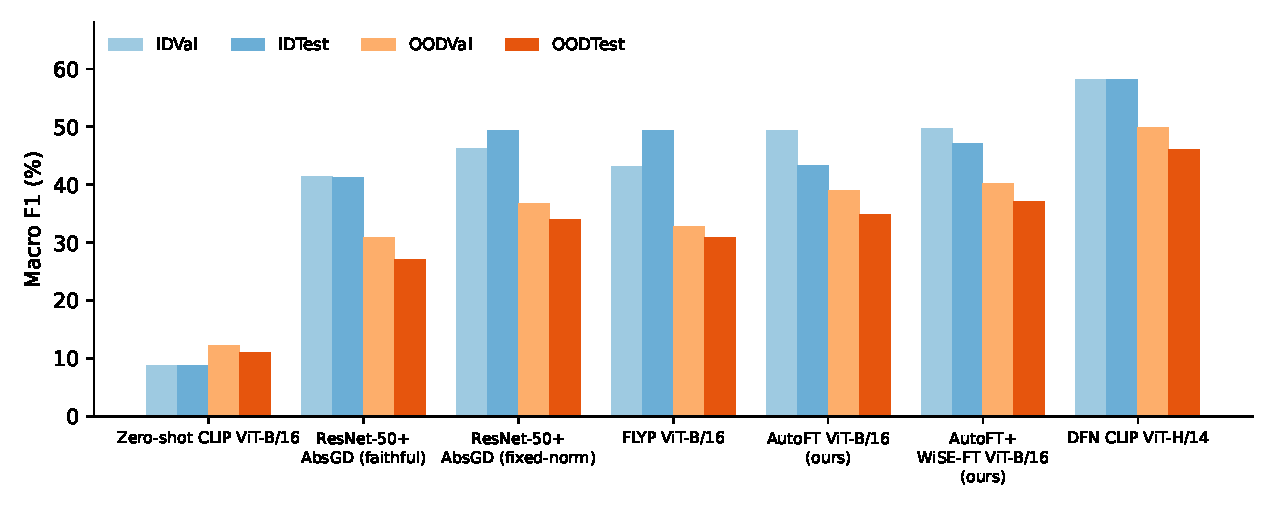
\includegraphics[width=\linewidth]{figures/baselines_macrof1.pdf}
  \caption{Macro F1 of the baseline family on the four official splits. CLIP fine-tunes
  dominate the ResNet baseline; every model drops on OOD splits relative to ID.}
  \label{fig:baselines}
\end{figure}

Three findings stand out. \textbf{(1) AutoFT reproduces the published pattern over FLYP.}
On the same ViT-B/16 backbone, AutoFT improves OOD-test macro F1 by $+4.0$ over FLYP,
and by $+6.3$ when interpolated with the zero-shot model (WiSE-FT, $\alpha$ selected on
ID-val only); \citet{choi2024autoft} report $+2.7$ and $+6.0$ on ViT-L/14@336. The
ensemble's benefit is strongly asymmetric---$+2.5$ OOD-test vs $+0.4$ ID-val---the same
asymmetry that carries the leaderboard entry from 48.7 to 52.0. \textbf{(2) Backbone and
objective both matter.} The ResNet-50 robust-optimizer baseline trails the CLIP
fine-tunes by 2--10 macro-F1 points depending on normalization variant, while the DFN
ViT-H/14---a larger CLIP---is the strongest single model at 46.1 OOD-test macro F1, in the
vicinity of FLYP's leaderboard number (46.0, ViT-L@336). \textbf{(3) The shift gap is
pervasive.} Every model loses 6--13 macro-F1 points from IDTest to OODTest
(Figure~\ref{fig:baselines}), which is exactly the regime where abstention should pay off.

Two caveats keep the comparison honest. The FLYP row was produced by a teammate's
independent implementation (lr $10^{-5}$, wd 0.2, batch 64, 20 epochs, seed 0, mixed
precision) rather than our CLI, and it reports IDTest $>$ IDVal---the opposite ordering
to all our runs---which suggests a possible IDVal/IDTest label swap in that eval harness;
we report its numbers as logged and will confirm the assignment. Absolute numbers sit
below the leaderboard because the leaderboard uses ViT-L/14@336; per our compute budget
all claims are relative to the FLYP row under near-identical conditions.

\section{Discussion}
Figure~\ref{fig:curves} shows the training dynamics behind the table: FLYP's contrastive
loss plateaus smoothly, the AutoFT fine-tune's ID-val macro F1 (monitored per epoch) drove
best-epoch selection, and the ResNet/DFN runs converge with clear train--validation gaps.

Beyond the results themselves, two engineering validations matter for a reproducibility
minded project. First, the AutoFT job was preempted by the cloud scheduler mid-run; the
per-epoch checkpoint/resume machinery continued from the last committed epoch, and the
restored best model reproduced its ID-val macro F1 exactly (0.4943) at evaluation time.
Second, an independent second evaluation pass reproduced every OOD number to four decimal
places, giving us confidence that the once-only OOD-test protocol is faithfully executed.

For the abstention lane, these results fix two design choices. The frozen classifier will
be AutoFT(+WiSE-FT): it is the strongest ViT-B/16 model and the leaderboard reference.
Following \citet{liang2024selectiveclassificationdistributionshifts}, we expect margins
to be near-parity with softmax on iWildCam, so the headroom for
\citet{heng2026know}'s $\Delta$-MDS/$\Delta$-KNN likelihood-ratio scores---and for our
augmentation-consistency extension---is a genuinely open question here; a negative result
would still be a well-instrumented finding. The DFN ViT-H/14 is an attractive alternative
backbone for a stretch lane if compute permits. Risks remain those identified in our
proposal: class imbalance (the ``empty'' class is 35\% of images), hard low-resolution
animals, and selectors that overfit training locations---hence the location-disjoint
split-A/B partition already in place.

\begin{figure}
  \centering
  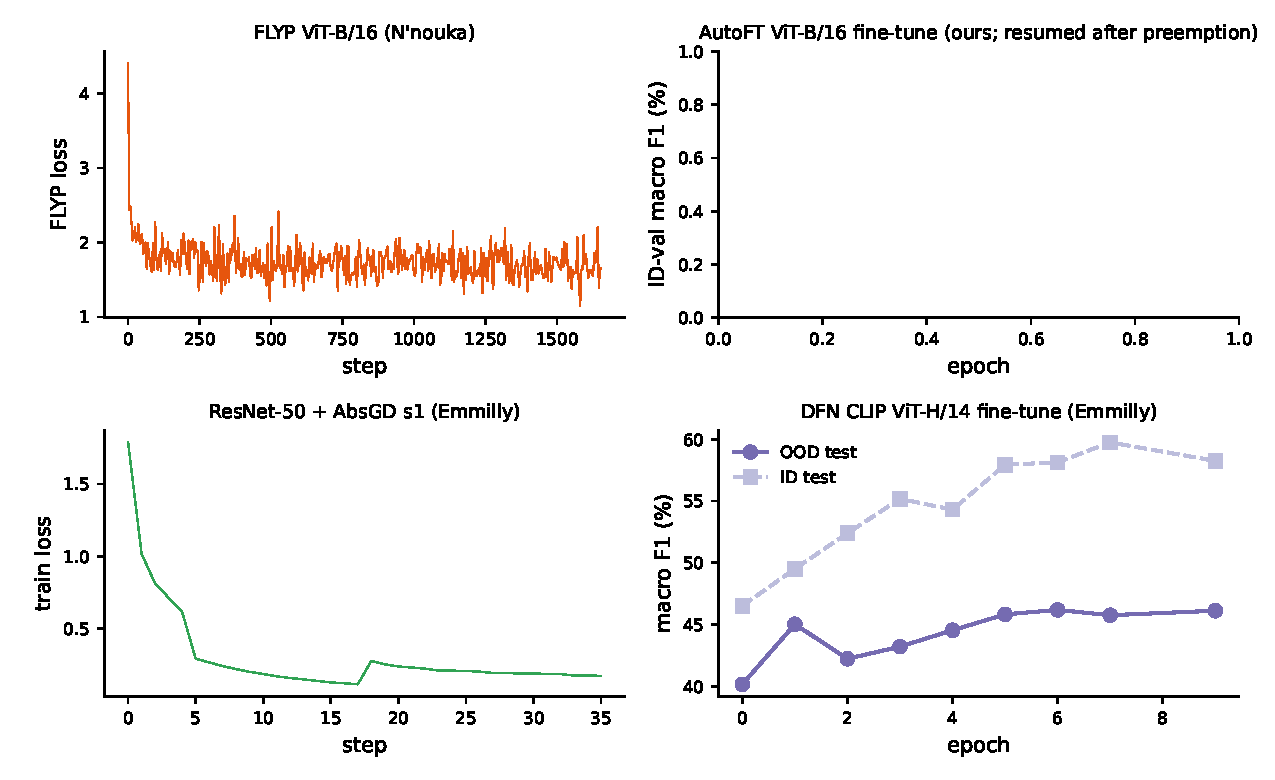
\includegraphics[width=\linewidth]{figures/training_curves.pdf}
  \caption{Training dynamics for one representative run per baseline family (from W\&B
  histories): FLYP contrastive loss, AutoFT per-epoch ID-val macro F1 (dashed line: the
  selected best), ResNet-50+AbsGD training loss, and DFN ViT-H/14 per-epoch ID/OOD-test
  macro F1.}
  \label{fig:curves}
\end{figure}

\section{Planned work}
\begin{itemize}
    \item Extract L2-normalized embeddings of the frozen AutoFT classifier on split-A/B
    locations (leakage-free protocol already materialized).
    \item Reproduce \citet{heng2026know}'s $\Delta$-MDS/$\Delta$-KNN + raw-logit-margin
    combination with MSP as the cheap comparator; produce risk--coverage curves and AURC
    on OOD val.
    \item Add the learned-combination and augmentation-consistency extensions; ablate
    each on the same frozen classifier; species- and location-level rejection analysis.
    \item (Stretch, if compute allows) leaderboard-faithful AutoFT on ViT-L/14@336 and/or
    the DFN ViT-H/14 as the frozen backbone.
\end{itemize}

\bibliographystyle{plainnat}
\bibliography{references}

\end{document}
